\subsection{Resultados con respecto al Tiempo de ejecuci\'on}

\subsubsection{Experimento 1}
\par El primer experimento consiste en correr el programa, variando la granularidad (en particular la del par\'ametro $m+1$, que determina la cantidad de puntos para cada \'angulo), con $ninst = 1$.
Se busca comparar el tiempo de ejecuci\'on de los distintos algoritmos para resolver un s\'olo sistema, con un \'unico t\'ermino independiente (a esto se debe $ninst = 1$).
Se espera que la Eliminaci\'on Gaussiana optimizada para banda se ejecute m\'as r\'apido que las otras, y que la Descomposici\'on LU sea la m\'as lenta, ya que se deben resolver dos sistemas en vez de uno s\'olo en el caso de Gauss.
El experimento consiste en correr 25 veces cada algoritmo con una serie de entradas en las cuales se mantienen constantes todos los par\'ametros excepto $m+1$ (es decir, variando s\'olo la granularidad). 
\par Se mide el tiempo que tardan en correr estas 25 iteraciones para cada entrada y m\'etodo de resoluci\'on del sistema lineal.
Se utiliza este m\'etodo de medici\'on en vez del promedio ya que ambos son similares (dan los mismos resultados, pero divididos o no por el tama\~no de la muestra), pero debido a la precisi\'on de la herramienta utiliza ($time$ de bash) preferimos dar el tiempo total para perder la menor precisi\'on posible.
\FloatBarrier

\subsubsection{Resultados del Experimento 1} 
\begin{figure}[ht]
\begin{center}
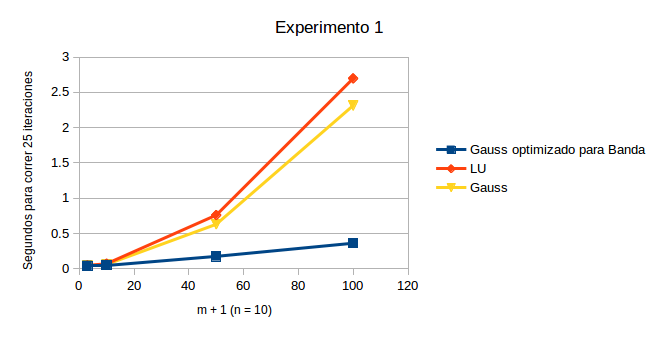
\includegraphics[width=0.8\columnwidth]{../src/experimentos/exp1-3/exp1figura}
\caption{Tiempo de ejecuci\'on en funci\'on del tama\~no de entrada, para ninst = 1}
\label{fig:figura1}
\end{center}
\end{figure}

\par Los resultados del experimento 1 se pueden observar en la figura \ref{fig:figura1}. \'Estos son los esperados: la Eliminaci\'on Gaussiana optimizada es la implementaci\'on m\'as r\'apida, seguida por la Eliminaci\'on Gaussiana (no optimizada), y la Descomposici\'on LU siendo la m\'as lenta.
Cabe destacar la forma cuadr\'atica de la curva del algoritmo de Gauss optimizado, comparada con la forma c\'ubica de las otras dos curvas. 
Ya que $n$ se mantiene constante, el ancho de la banda (que, como se mencion\'o previamente es $n+1$) tambi\'en se mantiene constante, y por ende la complejidad del algoritmo se vuelve $O(tamano de la matriz^2)$, en vez de $O(tamano de la matriz^3)$, y el resultado obtenido es lo esperado.

\FloatBarrier

\subsubsection{Experimento 2}

\par El segundo experimento consiste en correr el programa, con un mismo tama\~no de entrada, pero variando $ninst$. 
El prop\'osito de este experimento es observar como var\'ia el tiempo de ejecuci\'on de los distintos algoritmos para sistemas con varios t\'erminos independientes.
\par Se espera que LU sea m\'as r\'apido que Gauss, ya que s\'olo debe descomponer una vez al sistema y luego puede obtener la soluci\'on para distintos t\'erminos independientes solamente resolviendo
dos sistemas triangulares (que se hace en tiempo $O(tamano de la matriz^2)$. 
\par Sin embargo, la relaci\'on entre el tiempo de ejecuci\'on del algoritmo LU (que tiene un costo inicial de $O(tamano de la matriz^3)$, pero que al aumentar $ninst$, deber\'ia ser opacado por los costos de resolver m\'ultiples veces el sistema en $O(tamano de la matriz^2)$) y Gauss optimizado para Banda (que resuelve una sola vez el sistema, pero debe triangularlo cada vez en $O(tamano de la matriz^2)$) no es conocida de antemano; este tiempo es igual desde el punto de vista de la notaci\'on $O$ grande, pero las constantes escondidas resultar\'an en uno de los m\'etodos sobrepasando al otro.
\FloatBarrier

\subsubsection{Resultados del Experimento 2}


\begin{figure}[ht]
\begin{center}
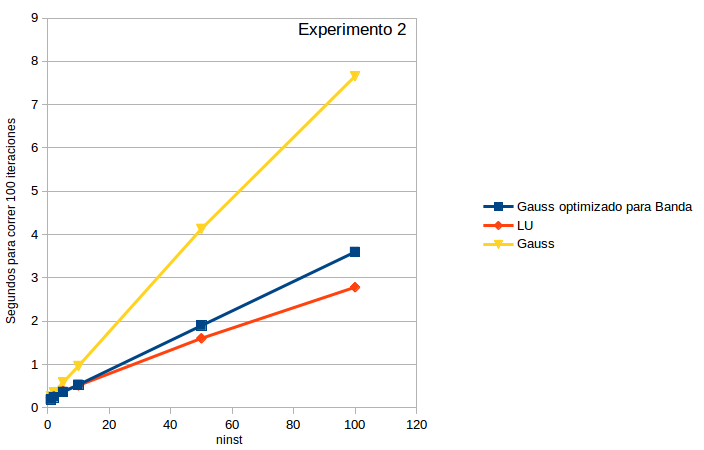
\includegraphics[width=0.8\columnwidth]{../src/experimentos/exp1-3/exp2figuratodos}
\caption{Tiempo de ejecuci\'on en funci\'on de ninst. Gr\'afico con todos los resultados del experimento.}
\label{fig:figura2}
\end{center}
\end{figure}

\begin{figure}[ht]
\begin{center}
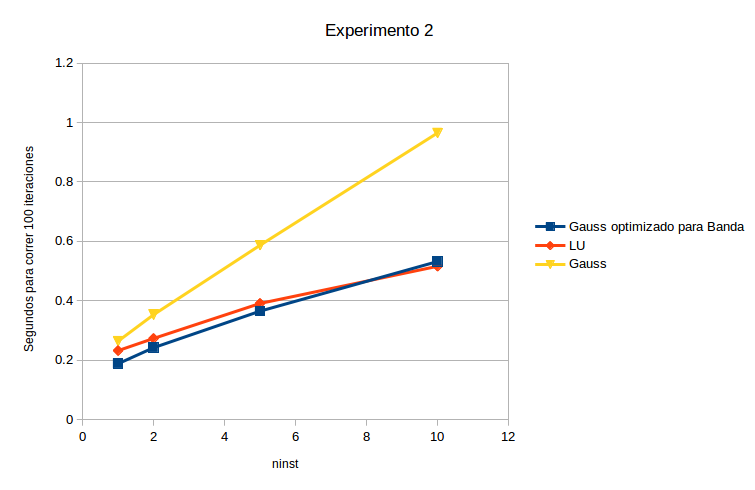
\includegraphics[width=0.8\columnwidth]{../src/experimentos/exp1-3/exp2figurahasta10}
\caption{Tiempo de ejecuci\'on en funci\'on de ninst. Gr\'afico con los valores hasta ninst = 10}
\label{fig:figura3}
\end{center}
\end{figure}


\par Los resultados del experimento 2 se pueden observar en las figuras \ref{fig:figura2} y \ref{fig:figura3} (esta \'ultima representa los mismos resultados que la anterior, pero s\'olo para $ninst\leq10$, para mayor claridad).
Si bien los resultados concernientes a la Eliminaci\'on Gaussiana son los esperados, la relaci\'on entre el tiempo de ejecuci\'on de LU y Gauss optimizado es interesante: para valores peque\~nos de $ninst$, Gauss optimizado es m\'as r\'apido, pero para valores grandes LU lo es.
Esto se debe a que resolver los sistemas de LU tiene un costo menor que triangular y resolver los sistemas utilizando Gauss optimizado; sin embargo, para valores peque\~nos de $ninst$, el costo c\'ubico de la Descomposici\'on LU tiene un mayor peso.

\FloatBarrier

\subsubsection{Experimento 3}
\par El experimento 3 consiste en correr los algoritmos, variando $m+1$ y $n$, pero manteniendo $(m+1)*n$ constante.
El prop\'osito de este experimento es observar como var\'ia el tiempo de ejecuci\'on de los algoritmos al variar s\'olo el ancho y el alto de la banda (que, como se demostr\'o previamente, equivalen a $n+1$), pero manteniendo constante la dimensi\'on de la matriz.
Se espera ver una clara diferencia en lo concerniente al algoritmo optimizado para banda. Los algoritmos de Gauss y LU, tienen una menor optimizaci\'on para banda (que fue detallada en la Introducci\'on Te\'orica), pero no se sabe de antemano cu\'an efectiva es.

\FloatBarrier

\subsubsection{Resultados del Experimento 3}

\begin{figure}[ht]
\begin{center}
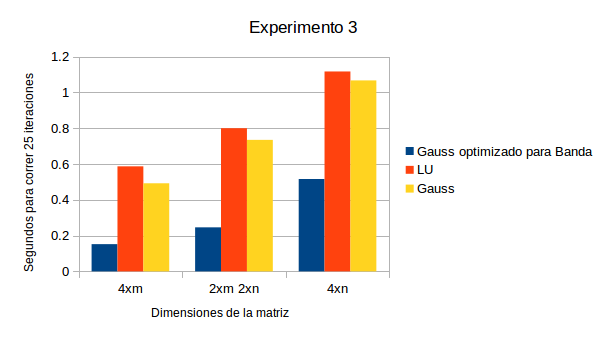
\includegraphics[width=0.8\columnwidth]{../src/experimentos/exp1-3/exp3figura}
\caption{Tiempo de ejecuci\'on para banda de distinto tama\~no, con dimensi\'on de la matriz constante.}
\label{fig:figura4}
\end{center}
\end{figure}

\par Los resultados del experimento 3 se pueden observar en la figura \ref{fig:figura4}. Como era de esperar, se incrementa el tiempo de ejecuci\'on del algoritmo de Gauss optimizado para banda al incrementar el ancho y alto de \'esta; sin embargo, es interesante notar que tambi\'en se incrementa el tiempo de ejecuci\'on de los otros dos algoritmos, y de forma considerable, lo que nos demuestra que la optimizaci\'on mencionada tiene un efecto significante sobre la velocidad de los m\'etodos.
\FloatBarrier

\subsection{Resultados con respecto a la Isoterma}

\subsubsection{Experimento 4}
\par En este experimento se busca comparar los resultados obtenidos en las temperaturas del horno y en el cálculo de la isoterma variando la granularidad de los radios. Para ello tomaremos dos inputs de entrada con los mismos valores de temperatura interna y externa (1500 y 0 respectivamente), mismos radio interno e externo (10 y 100) y misma cantidad de ángulos (30). El primero (4a) dividirá el horno en 10 radios, mientras que el segundo (4b) lo hará en 100. Conjeturamos que al tener más granularidad con respecto a los radios, se obtendrá una isoterma con menos imperfecciones, permitiendo evaluar la peligrosidad de manera más precisa.
\FloatBarrier

\subsubsection{Resultados del experimento 4}

\begin{figure}[ht]
\begin{center}
\subfigure [4a - 10 radios] {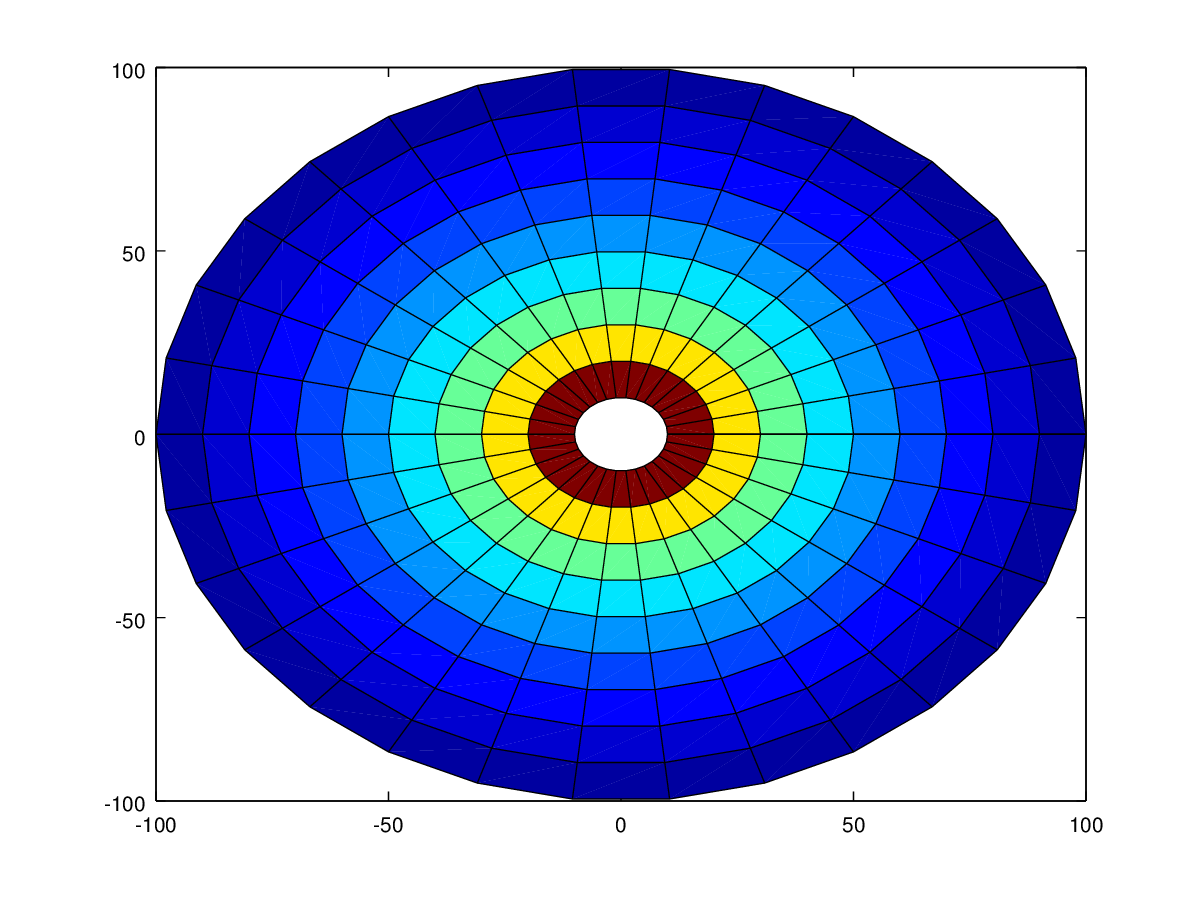
\includegraphics[width=0.49\columnwidth]{../src/experimentos/exp4/calor4A.png}}
\subfigure [4b - 100 radios] {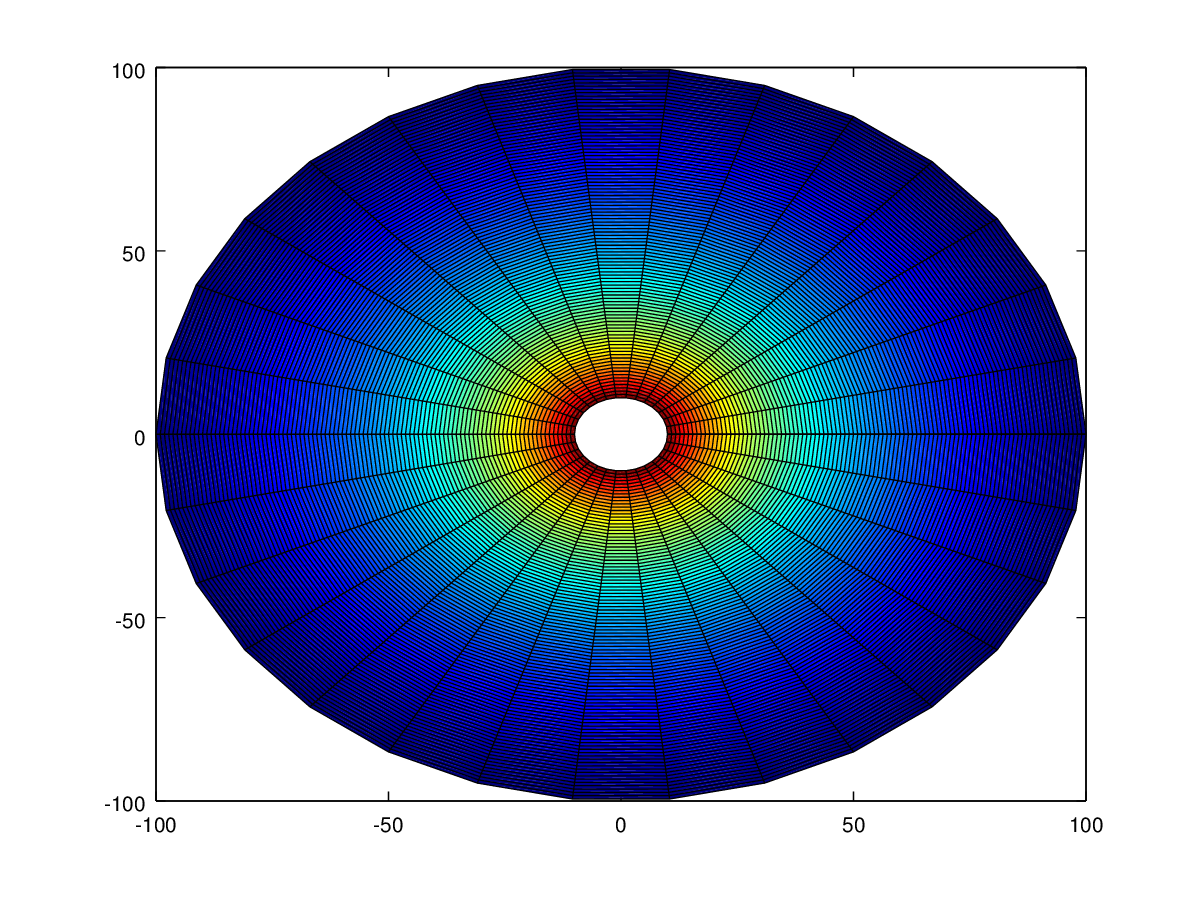
\includegraphics[width=0.49\columnwidth]{../src/experimentos/exp4/calor4b.png}}
\caption{Experimento 4, gráfico de calor}
\end{center}
\end{figure}

\begin{figure}[ht]
\begin{center}
\subfigure [4a - 10 radios] {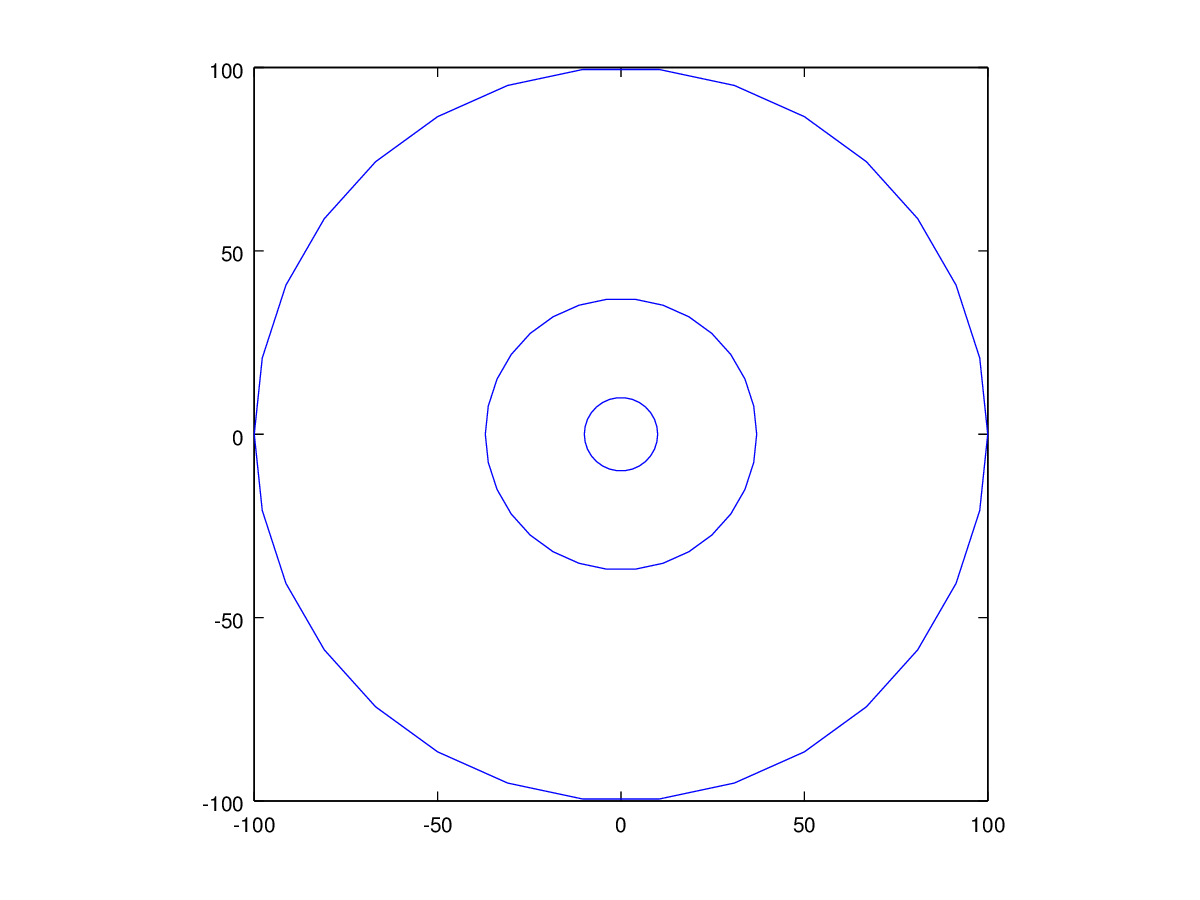
\includegraphics[width=0.49\columnwidth]{../src/experimentos/exp4/iso4A.png}}
\subfigure [4b - 100 radios] {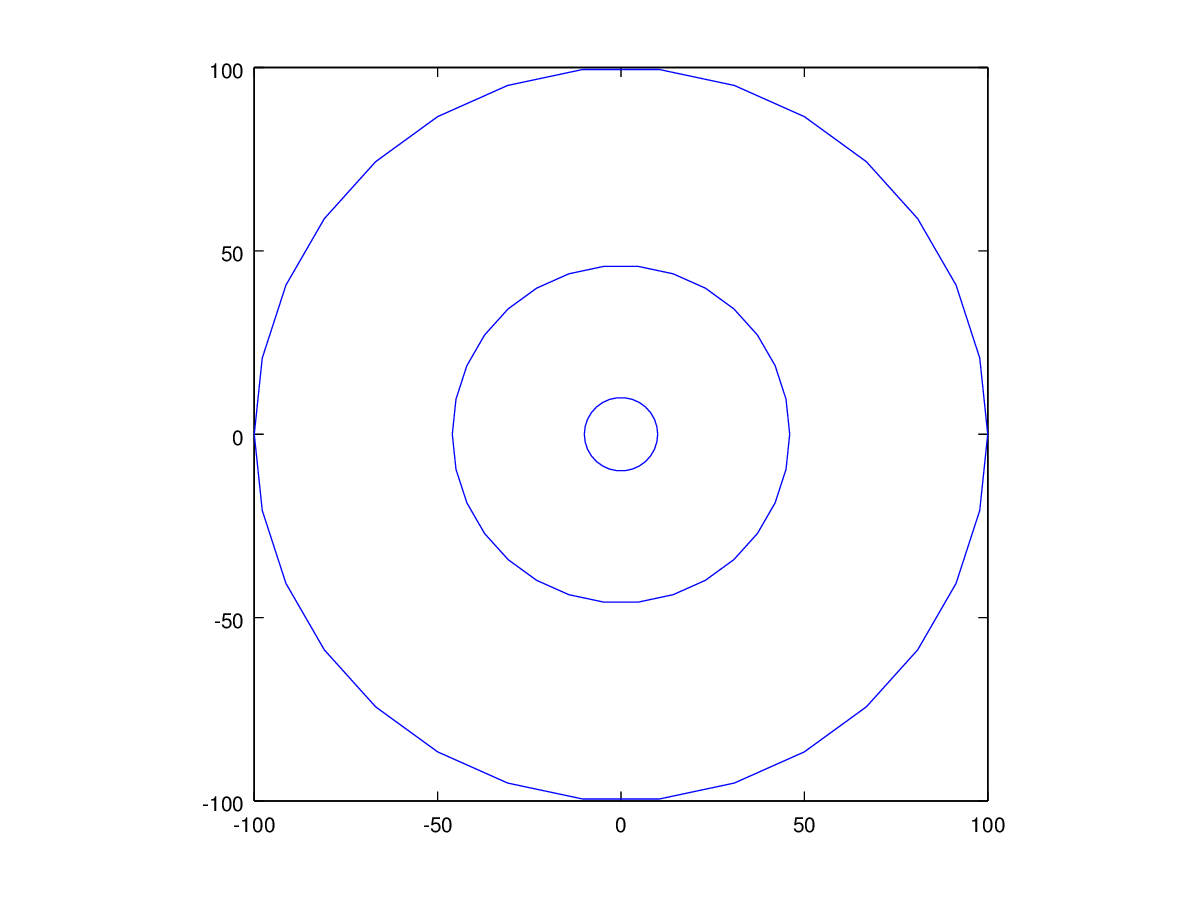
\includegraphics[width=0.49\columnwidth]{../src/experimentos/exp4/iso4b.png}}
\caption{Experimento 4, gráfico de isoterma}
\end{center}
\end{figure}

\par Como se ve en los gráficos, se observa mayor precisión al aumentar la granularidad. La isoterma en el caso que toma mayor cantidad de radios se acerca al borde externo, lo que podría indicar que un test de peligrosidad podría llegar a dar un falso negativo si no se toma la cantidad adecuada de radios, provocando una falla grave en el sistema.

\subsubsection{Experimento 5}

\par Análogamente, en este experimento se observará como varían las temperaturas y la isoterma al modificar la cantidad de ángulos de entrada, manteniendo las demás variables constantes.

\FloatBarrier

\subsubsection{Resultados del experimento 5}

\begin{figure}[ht]
\begin{center}
\subfigure [5a - 10 ángulos] {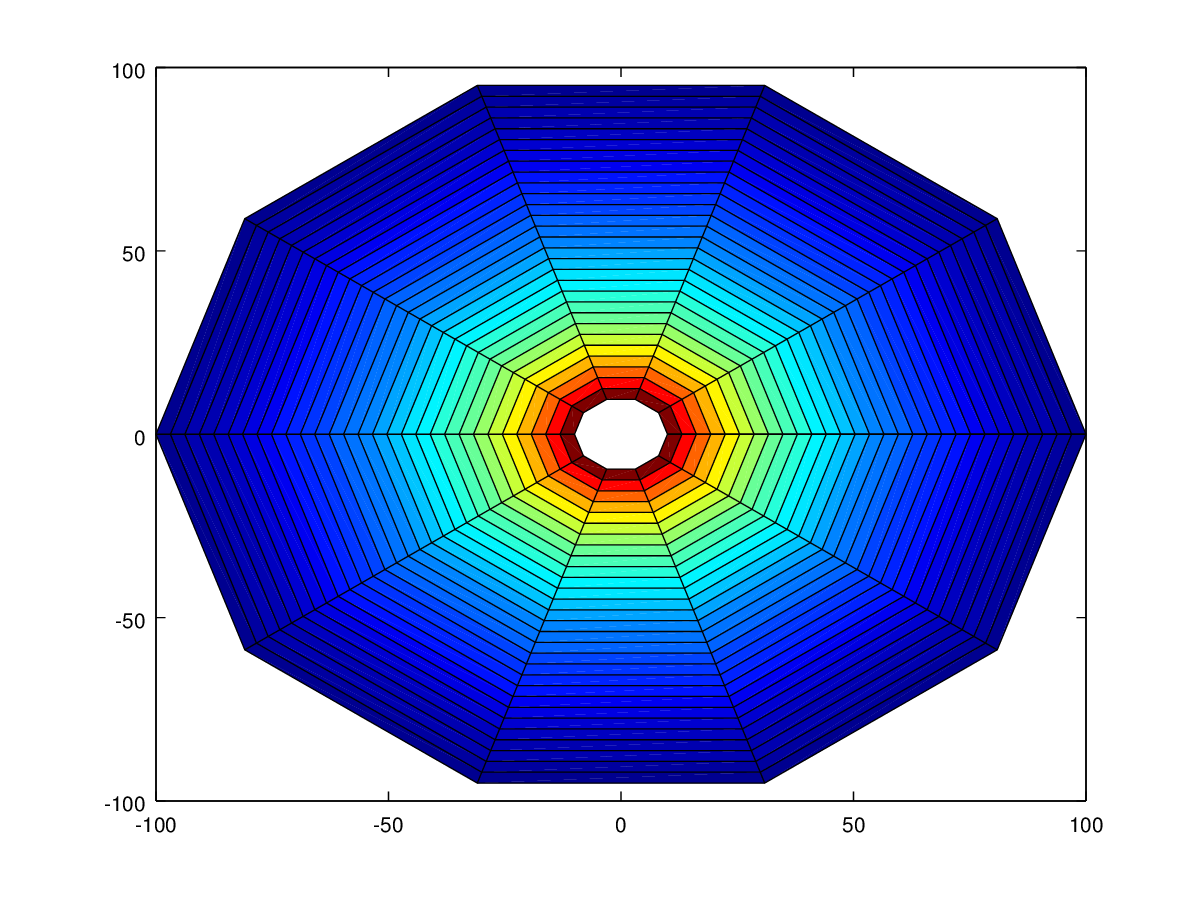
\includegraphics[width=0.49\columnwidth]{../src/experimentos/exp5/calor5a.png}}
\subfigure [5b - 100 ángulos] {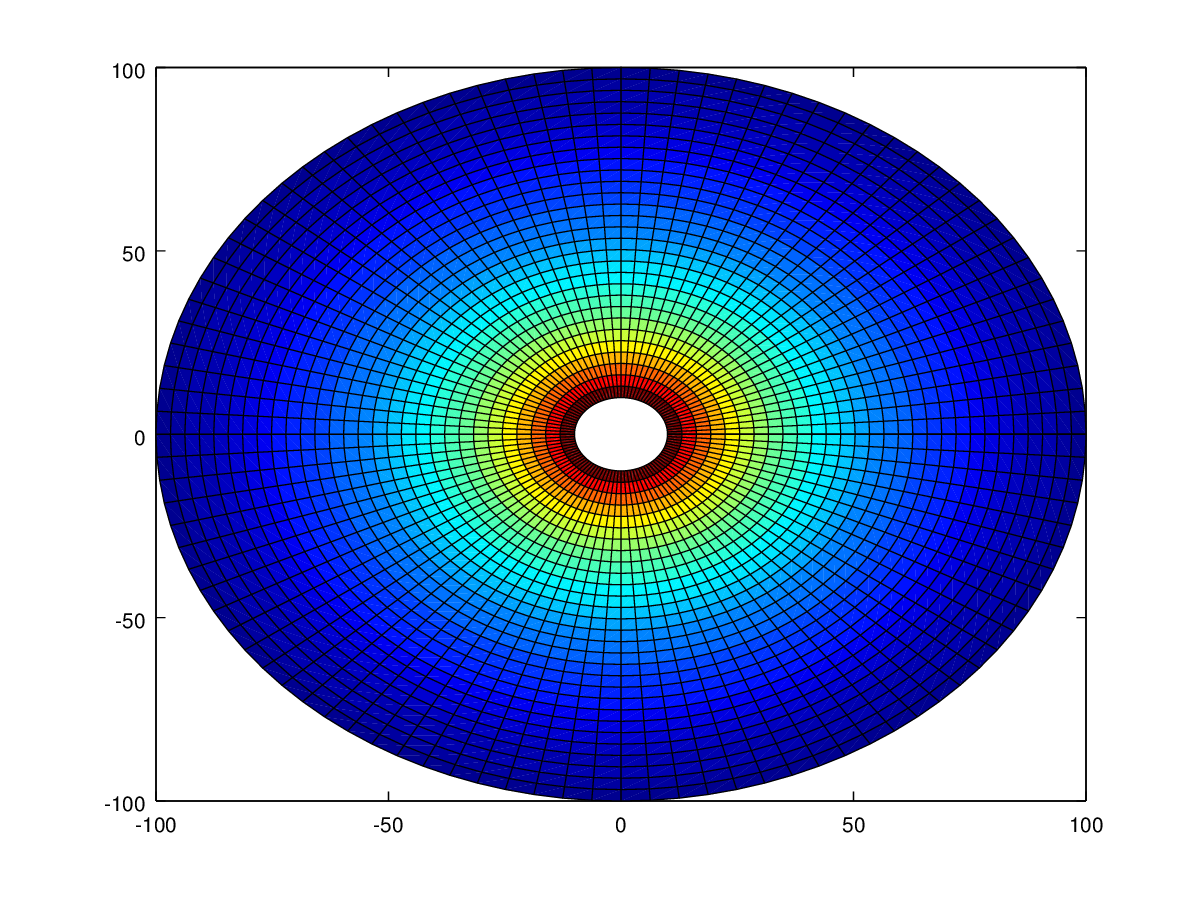
\includegraphics[width=0.49\columnwidth]{../src/experimentos/exp5/calor5b.png}}
\caption{Experimento 5, gráfico de calor}
\end{center}
\end{figure}

\begin{figure}[ht]
\begin{center}
\subfigure [5a - 10 ángulos] {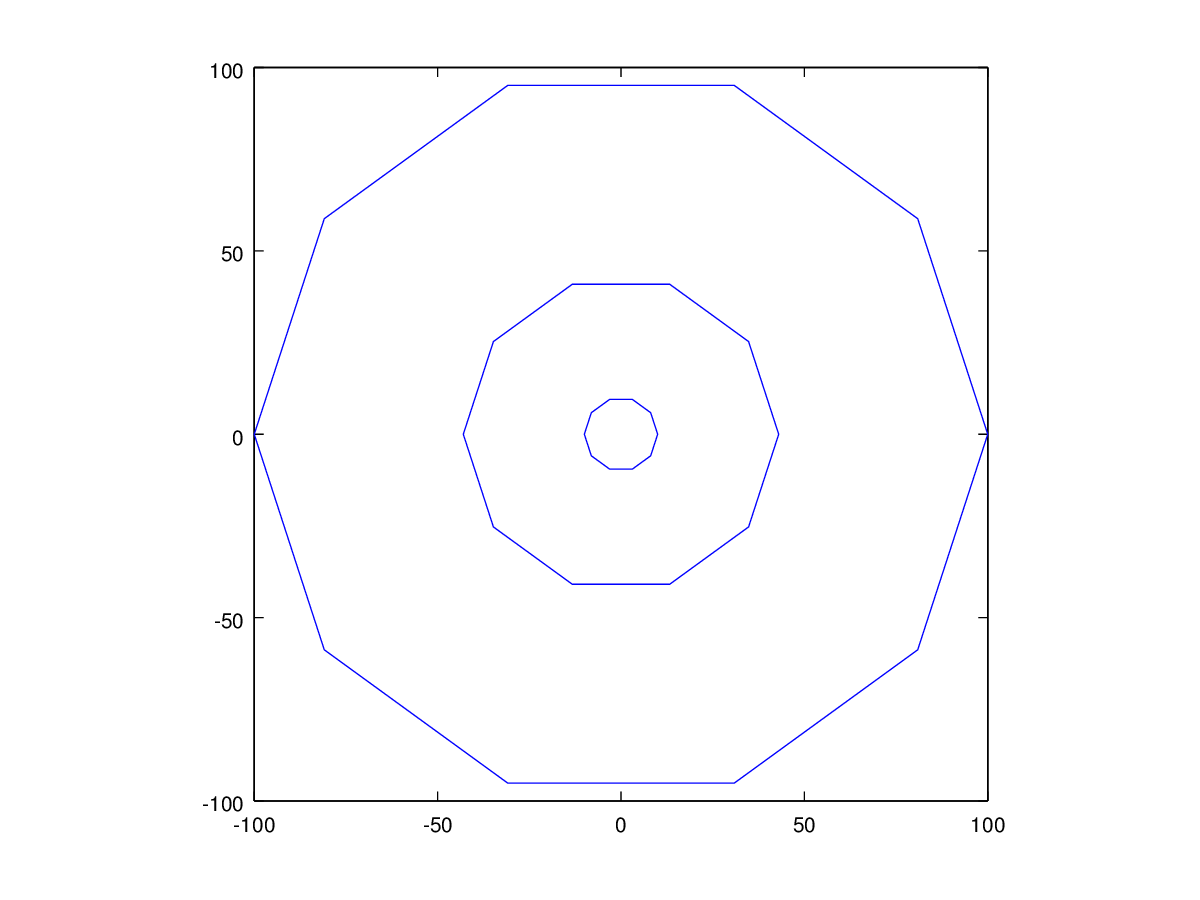
\includegraphics[width=0.49\columnwidth]{../src/experimentos/exp5/iso5a.png}}
\subfigure [5b - 100 ángulos] {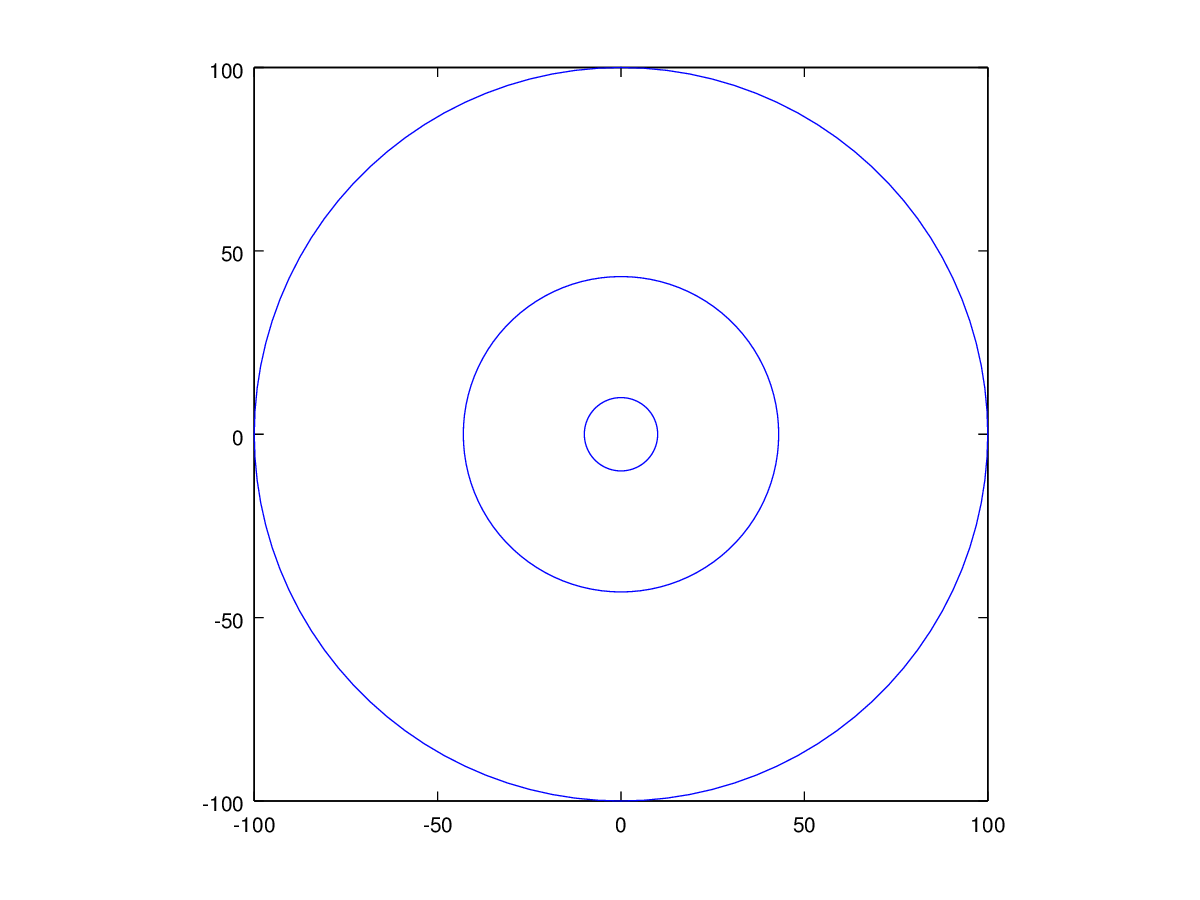
\includegraphics[width=0.49\columnwidth]{../src/experimentos/exp5/iso5b.png}}
\caption{Experimento 5, gráfico de isoterma}
\end{center}
\end{figure}

\par Al igual que en el experimento anterior, la precisión aumenta al aumentar la cantidad de ángulos. En este caso la forma de la isoterma se ve que se asemeja a un círculo al aumentar la granularidad en los ángulos, que es la verdadera forma del horno. Esto es importante ya que decidir si se encuentra en condiciones de peligro con una isoterma tan deformada podría dar resultados incorrectos.

\subsubsection{Experimento 6}

\par Por último, en este experimento se desea comparar los resultados al aumentar la granularidad en ambas variables (radios y ángulos), con el objetivo de determinar cuál de ellas es más importante, refiriéndonos a su granularidad, a la hora de lograr una isoterma que permita calcular la peligrosidad de manera correcta.


\subsubsection{Resultados del experimento 6}

\begin{figure}[ht]
\begin{center}
\subfigure [6a - 10 radios y 10 ángulos] {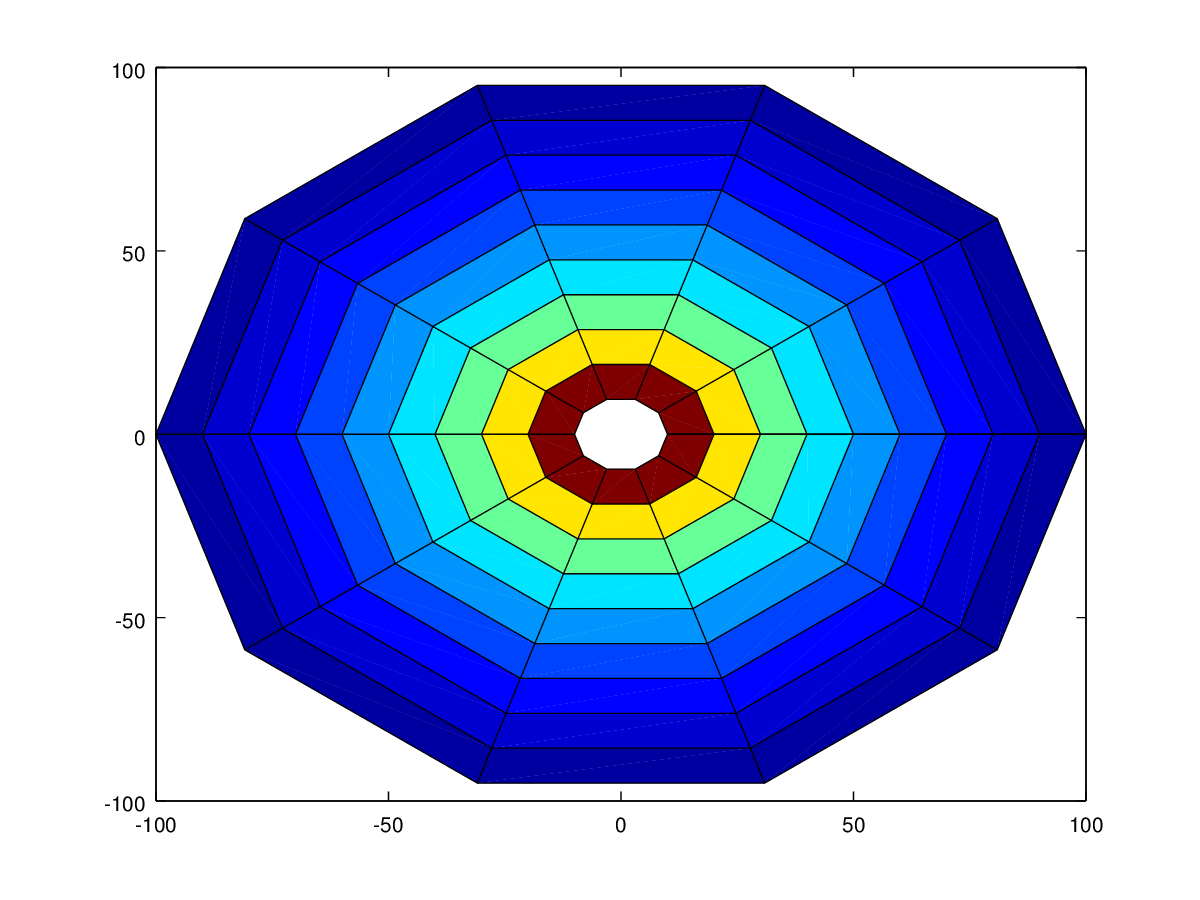
\includegraphics[width=0.49\columnwidth]{../src/experimentos/exp6/calor6a.png}}
\subfigure [6b - 100 radios y 100 ángulos] {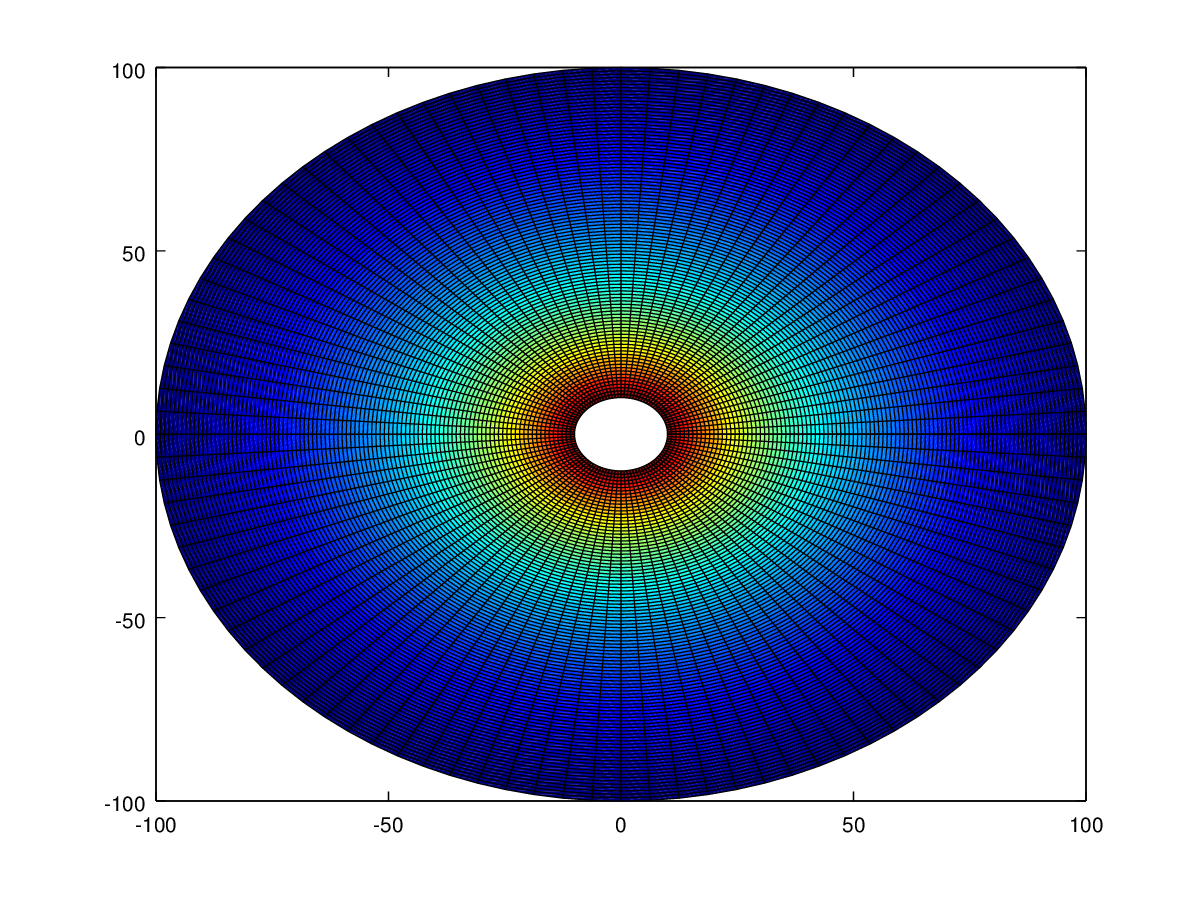
\includegraphics[width=0.49\columnwidth]{../src/experimentos/exp6/calor6b.png}}
\caption{Experimento 6, gráfico de calor}
\end{center}
\end{figure}

\begin{figure}[ht]
\begin{center}
\subfigure [6a - 10 radios y 10 ángulos] {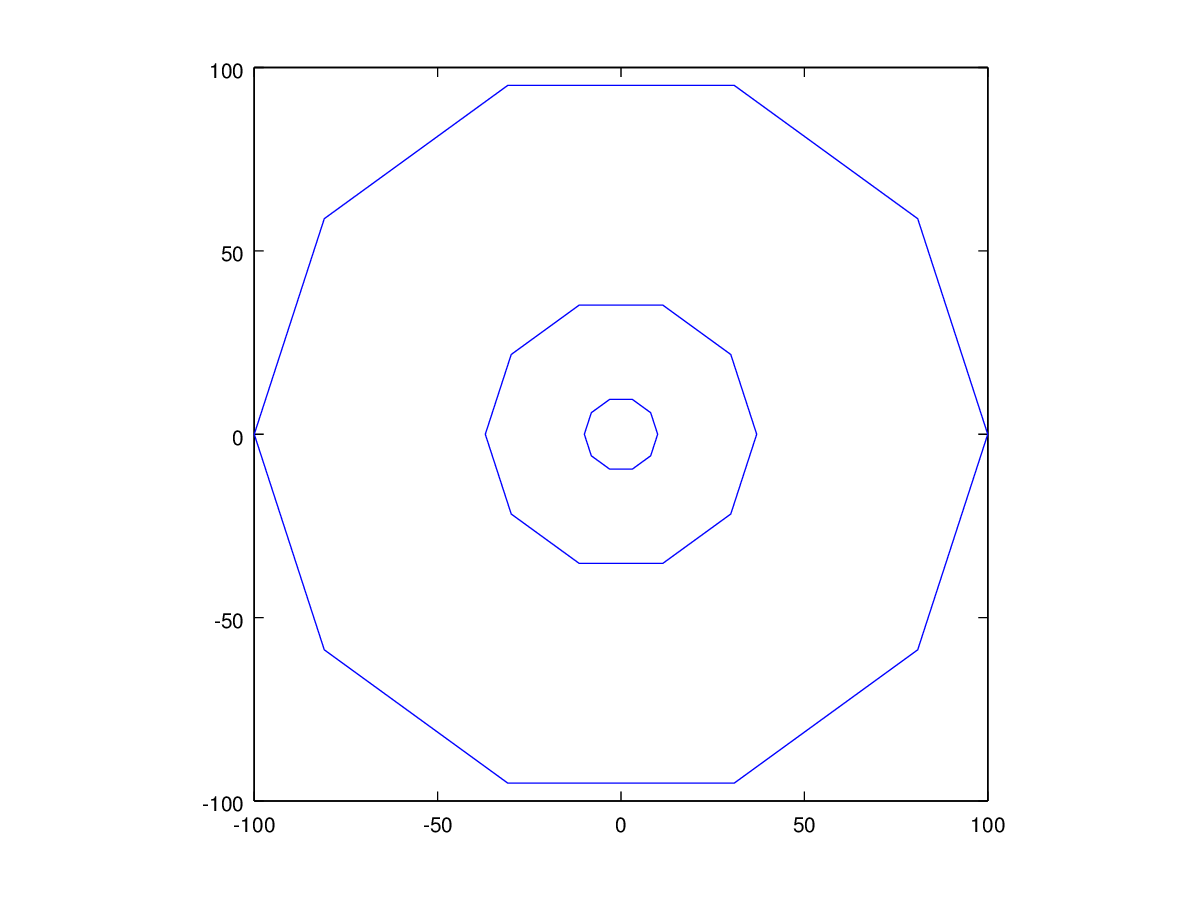
\includegraphics[width=0.49\columnwidth]{../src/experimentos/exp6/iso6a.png}}
\subfigure [6b - 100 radios y 100 ángulos] {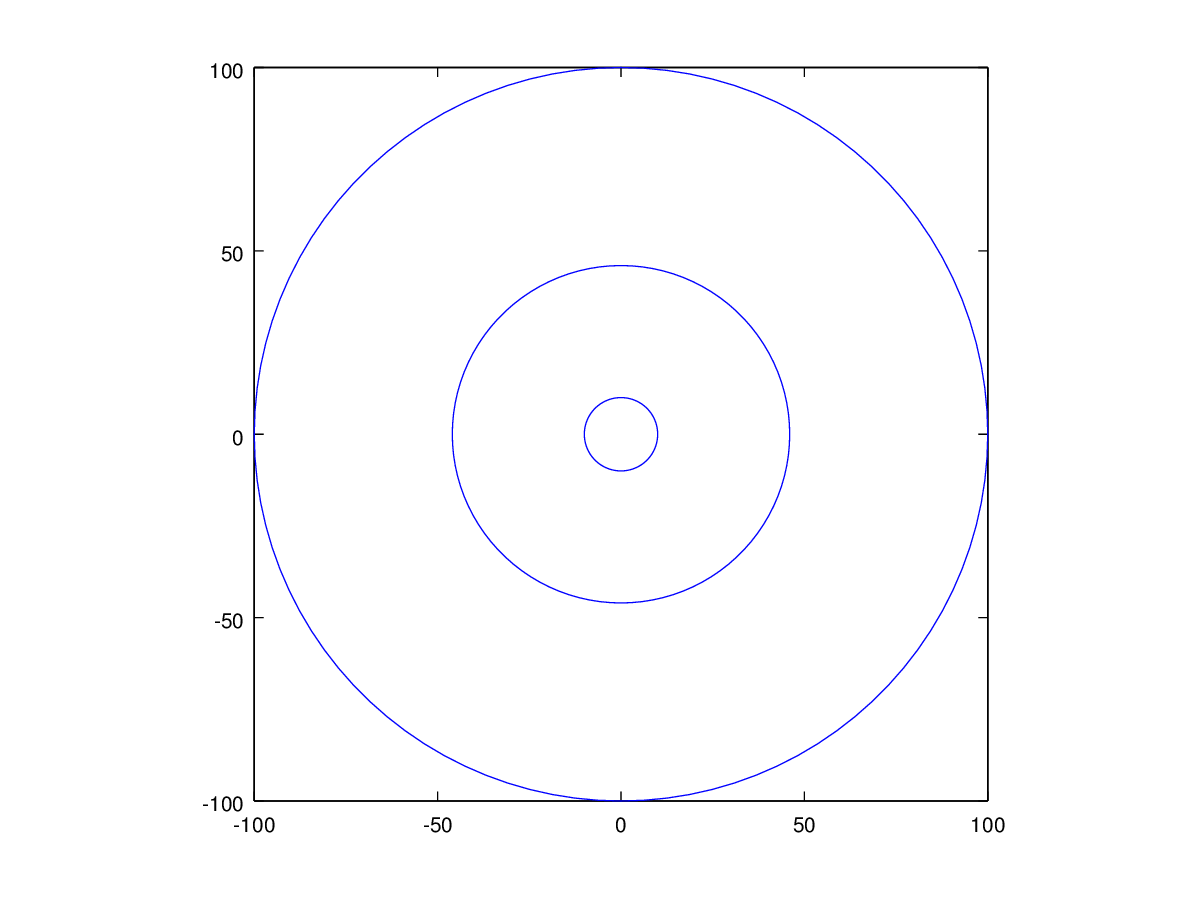
\includegraphics[width=0.49\columnwidth]{../src/experimentos/exp6/iso6b.png}}
\caption{Experimento 6, gráfico de isoterma}
\end{center}
\end{figure}

\par Concluimos que la granularidad es una variable muy importante a la hora de determinar las temperaturas del horno, más allá de que aumente la complejidad temporal del algoritmo. Como se pudo ver en estos experimentos, disminuir la granularidad de alguna de las variables puede producir resultados incorrectos a la hora de calcular peligrosidad. Además, vemos que ambas variables (radios y ángulos) tienen igual importancia, a pesar de que el gráfico para poca cantidad de ángulos se vea más deformado a simple vista.

\subsubsection{Experimento 7}
\par Contamos con distintas formas de calcular la isoterma:
\begin{itemize}
\item Redondear al punto mas cercano.
\item Promediar el punto entre los mas cercanos.
\end{itemize}

\par Creemos que cuanto mayor distancia entre puntos de discretización, mayor va a ser la distancia entre el punto calculado por el procedimiento 1 y el verdadero valor de radio de la isoterma. En cambio con el procedimiento 2 nos aseguramos acercarnos 'un poco mas' (mas allá de la distancia entre radios).

\subsubsection{Primera entrada para el experimento 7}
\par Para simular este caso particular vamos a tomar un estado donde el radio interno es 10mts y el externo es 10000mts. Tomamos tan solo 30 radios, por lo que la distancia entre radios es de 333mts. Tomamos temperaturas internas alternantes entre 5500, 1000 y 550 para lograr una isoterma no circular y variable. Planteamos como hipótesis que en el caso del procedimiento 1 la isoterma va a ser poco variable, y que, en caso de verse un salto, va a ser brusco (de 333mts) entre cada punto. Mientras que con el procedimiento 2 van a poder notarse mas cambios, pero mas leves, ya que al ir promediando va a variar entre puntos intermedios (menores a 333mts).

\subsubsection{Resultados para la primera entrada para el experimento 7}

\begin{figure}[ht]
\begin{center}
\subfigure [Procedimiento 1] {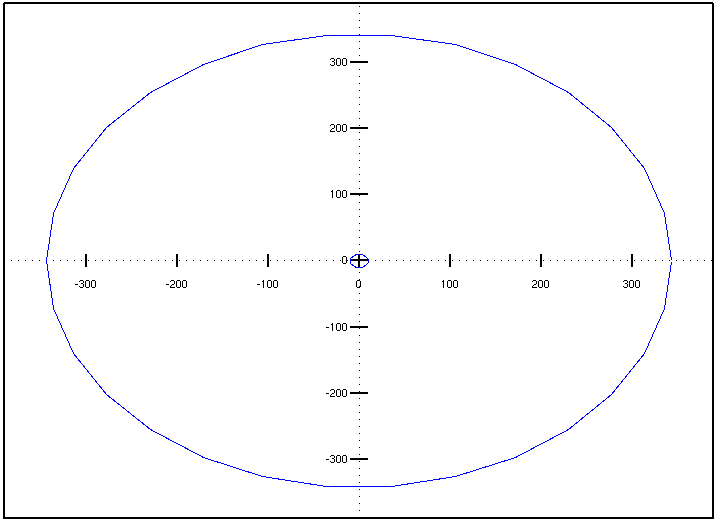
\includegraphics[width=0.49\columnwidth]{../src/experimentos/exp7/se_pudrio_todo/1/isoterma.png}}
\subfigure [Procedimiento 2] {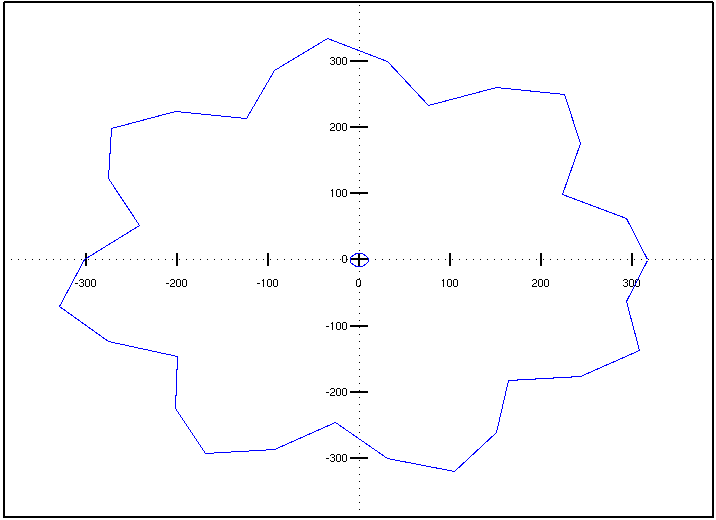
\includegraphics[width=0.49\columnwidth]{../src/experimentos/exp7/promedio/1/isoterma.png}}
\caption{Experimento 7, primera entrada}
\end{center}
\end{figure}

\par En los gráficos se puede notar la diferencia entre los resultados del procedimiento 1 y el 2. En el caso del 1, al mantenerse la isoterma cerca del radio 343mts se redondea tomando el punto 343mts. Esto se da en todos los ángulos, por lo que se obtiene una isoterma circular. Mientras que en el caso del procedimiento 2 se pueden distinguir los cambios y variaciones de la isoterma acercándose por valores intermedios de los radios, consiguiéndose así saltos leves.

\subsubsection{Segunda entrada para el Experimento 7}
\par Vamos a modificar la entrada dejando solo temperaturas externas variables entre 1500 y 1200. Creemos que esto no va a modificar el gráfico de la isoterma según el procedimiento 1, ya que si disminuimos la diferencia de las temperaturas las isotermas de los diferentes ángulos deberían ocupar radios mas cercanos entre sí. Si creemos que va a cambiar el gráfico de la isoterma del procedimiento 2, ya que si hay poca diferencia entre las temperaturas externas debería acercarse un círculo.

\subsubsection{Resultados para la segunda entrada para el Experimento 7}

\begin{figure}[ht]
\begin{center}
\subfigure [Procedimiento 1] {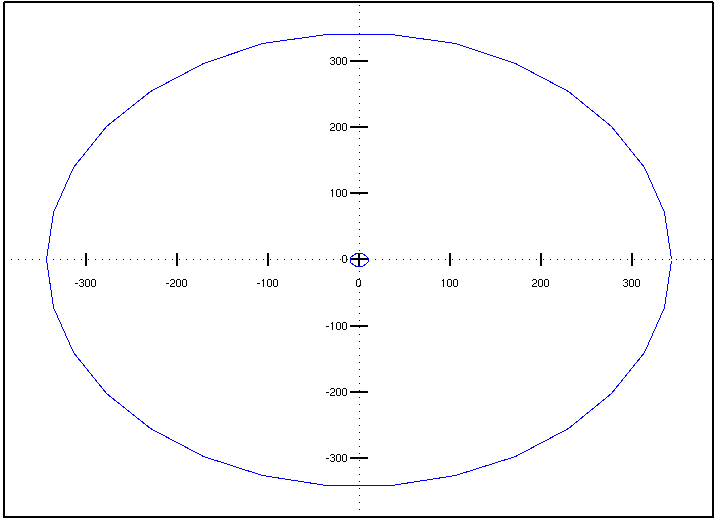
\includegraphics[width=0.49\columnwidth]{../src/experimentos/exp7/se_pudrio_todo/2/isoterma.png}}
\subfigure [Procedimiento 2] {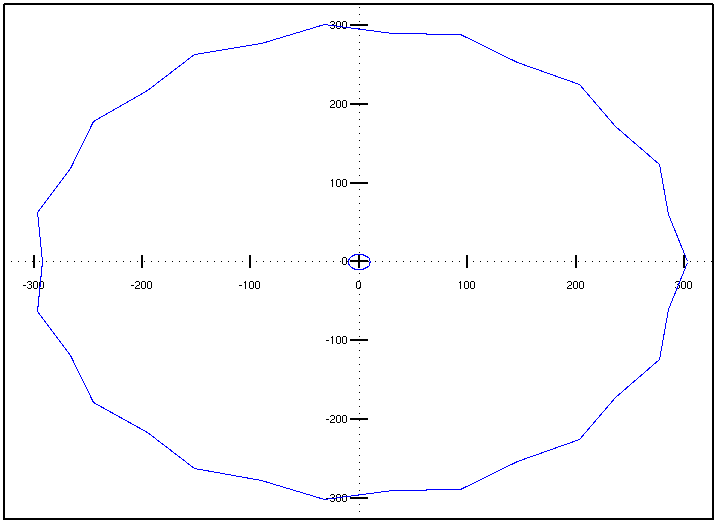
\includegraphics[width=0.49\columnwidth]{../src/experimentos/exp7/promedio/2/isoterma.png}}
\caption{Experimento 7, segunda entrada}
\end{center}
\end{figure}

\par En el gráfico del procedimiento 1, podemos notar que la isoterma tiene forma circular (igual que en A), debido a la poca diferencia entre temperaturas externas y que redondeamos su valor. En cambio en el caso del procedimiento 2 notamos una gran diferencia con respecto al gráfico del A. Como pudimos predecir, al acercar las temperaturas externas entre sí los puntos de la isoterma se posicionan mas cerca y ya no veos saltos tan bruscos. Lo que si podemos ver es que los valores de la isoterma varían entre 2 puntos (al igual que las temperaturas externas).

\subsubsection{Experimento 8}
\par Creemos que podríamos ahorrar tiempo si ejecutamos un estado con pocos radios y usando el procedimiento 2 para calcular la isoterma en vez de usar el procedimiento 1 con mas granularidad de radios. Para esto tomamos un estado con temperaturas externas variables entre 1500 y 1000 grados y vamos a calcular su isoterma 300 utilizando el procedimiento 2 con 10 radios. También calcularemos la misma isoterma utilizando el procedimiento 1 con 20 y 100 radios y compararemos los resultados para ver si podemos aproximar la isoterma utilizando el procedimiento 2 con poca granularidad de radios.

\subsubsection{Resultados del Experimento 8}

\begin{figure}[ht]
\begin{center}
\subfigure [Procedimiento 2 con 10 radios] {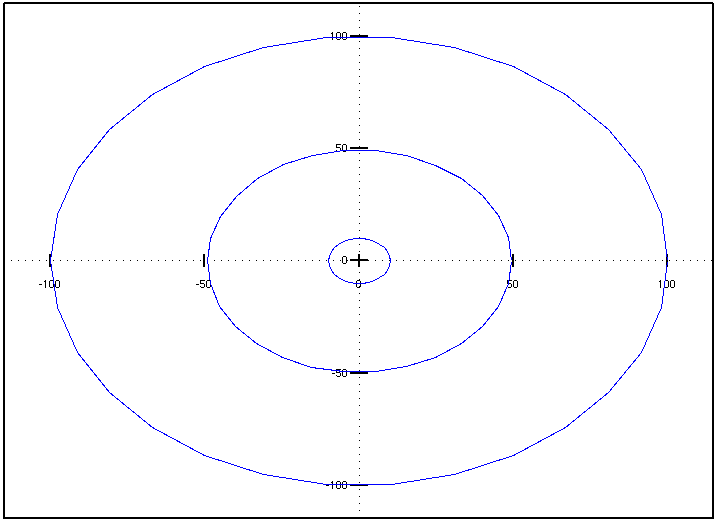
\includegraphics[width=0.49\columnwidth]{../src/experimentos/exp8/promedio/10/isoterma.png}}
\subfigure [Procedimiento 1 con 100 radios] {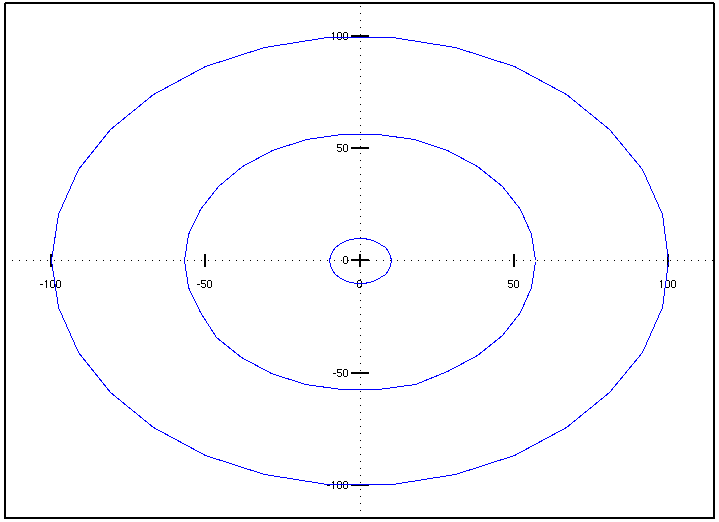
\includegraphics[width=0.49\columnwidth]{../src/experimentos/exp8/gran_spt/100/isoterma.png}}
\caption{Experimento 8}
\end{center}
\end{figure}

\par Como vemos en los gráficos, la isoterma obtenida con el procedimiento 2 nos sirven para aproximar (a grandes rasgos) la posición de la isoterma, pero tomando en cuenta que calcular la isoterma con el procedimiento 1 y 100 radios no nos llevó un tiempo relevante podemos calcularla de esta forma y aproximar mucho mejor la isoterma (sin necesidad de mucho mas tiempo). Así concluimos que nuestro primer pensamiento de que se podía aproximar la isoterma con rapidéz utilizando el procedimiento 2 era correcta, pero solo a grandes rasgos. Y teniendo en cuenta lo dicho antes podemos utilizar el procedimiento 1 sin necesidad de pagar con gran tiempo de ejecución.


\subsection{Resultados con respecto a la Peligrosidad}

\subsubsection{Experimento 9}

\par En este experimento se buscará comparar dos métodos implementados para decidir la peligrosidad de un horno a partir de la isoterma 500.
\par El primero, tan solo se fija si alguno de los puntos de la isoterma 500 sobrepasa una distancia predeterminada al radio externo:

\lstset{language=C++, breaklines=true, basicstyle=\footnotesize}
\begin{lstlisting}[frame=single]
bool estaEnPeligro (vector<double>& isoVec, int ri, int re, double indiceDePeligro)
{
    double sePudrioTodo = ((double) re - ri) * indiceDePeligro;
    for (int i = 0; i < isoVec.size(); i++)
    {
        if (isoVec [i] >= sePudrioTodo) return true;
    }
    return false;
}
\end{lstlisting}

\par El segundo algoritmo, en cambio, calcula la cantidad de puntos en peligro y la compara con la cantidad total de puntos en la circunsferencia, calificándolo como en peligro si éste supera el 40\%. Seleccionamos uno de los casos bordes para mostrar la diferencia entre los métodos, donde la mitad izquierda del horno es más fría (quizás por algún mecanismo de ventilación o enfriamiento) que la de la derecha.

%\lstset{language=C++, breaklines=true, basicstyle=\footnotesize}
%\begin{lstlisting}[frame=single]
%bool estaEnPeligroPromedio (vector<double>& isoVec, int ri, int re, double indiceDePeligro)
%{
%    double sePudrioTodo = ((double) re - ri) * indiceDePeligro;
%    int peligrosos = 0;
%    for (int i = 0; i < isoVec.size(); i++)
%    {
%        if (isoVec [i] >= sePudrioTodo) peligrosos++;
%    }
%    if (peligrosos/isoVec.size() >= 0.4 ){
%        return true;
%    }else{
%        return false;
%    }
%}
%\end{lstlisting}

\subsubsection{Resultados del experimento 9}

\begin{figure}[ht]
\begin{center}
\subfigure [] {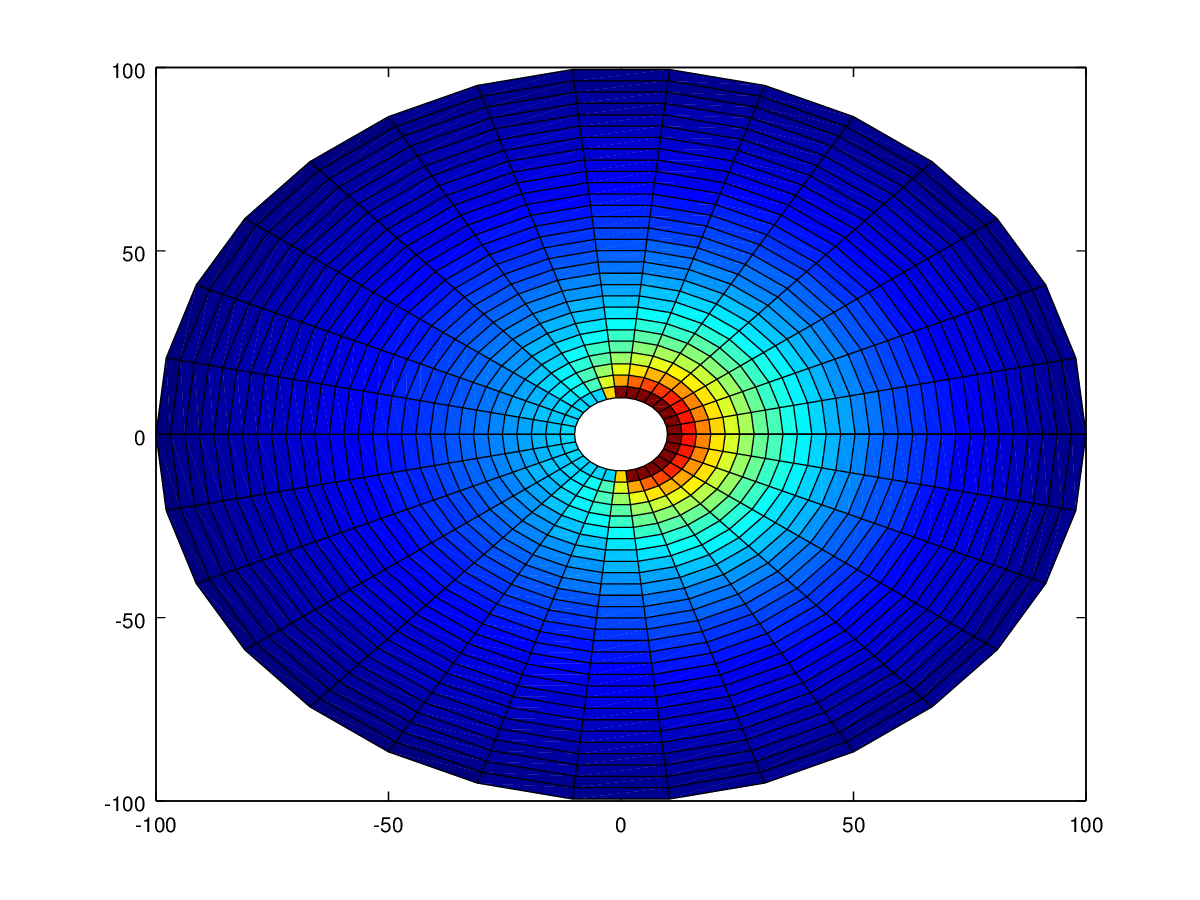
\includegraphics[width=0.5\columnwidth]{../src/experimentos/exp9/promedio/calor01.png}}
\subfigure [] {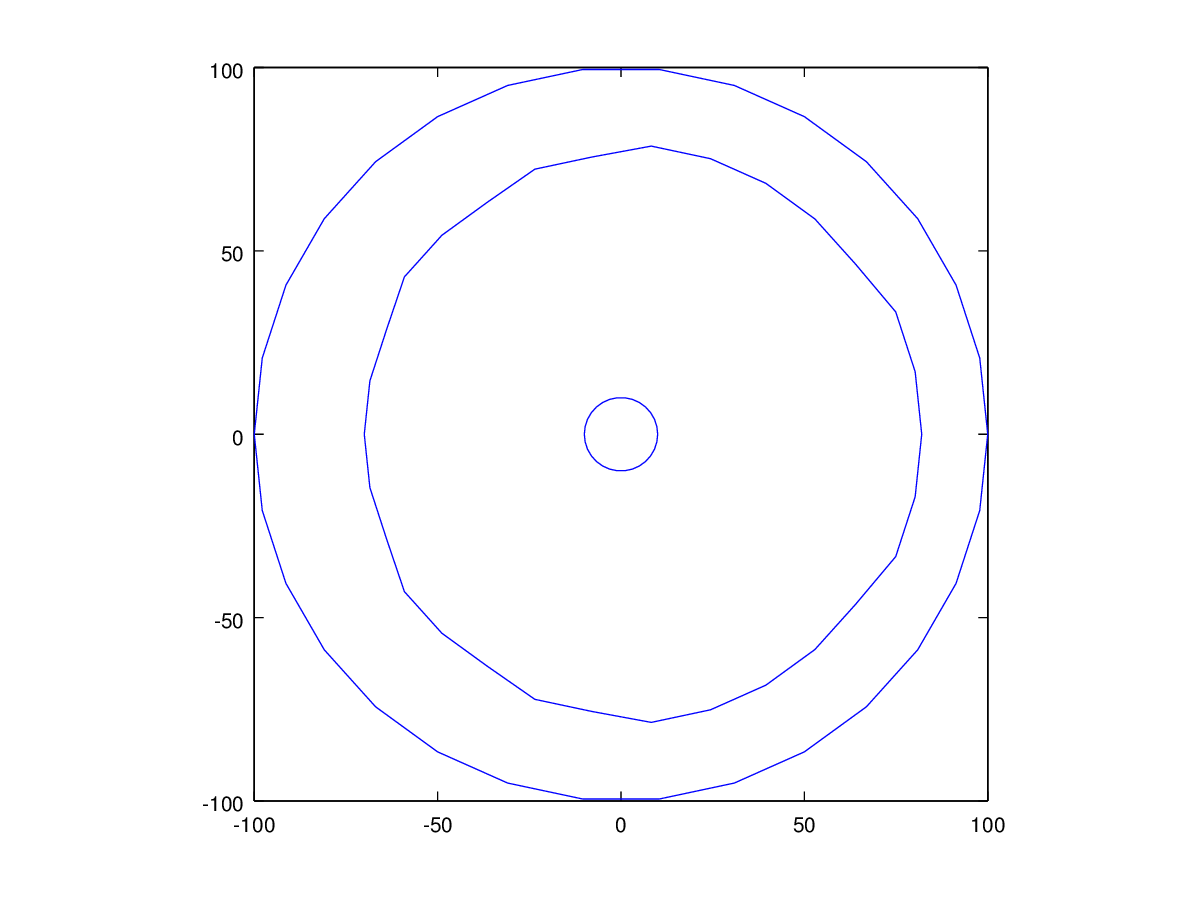
\includegraphics[width=0.49\columnwidth]{../src/experimentos/exp9/promedio/iso01.png}}
\caption{Experimento 9}
\end{center}
\end{figure}

\par estaEnPeligro da PELIGRO
\par estaEnPeligroPromedio da No esta en peligro

\par Para casos bordes como el mostrado en la figura 15, donde el horno tiene temperaturas más frías en un sector que en otro, los resultados de los métodos difieren. Quedará por decidir cuál de los dos es el más convieniente para cada situación: el primero, si nos encontramos en una situación crítica donde el menor exceso de temperatura pueda significar un grave problema; o el segundo, cuando la situación pueda ser más controlable si sólo una parte del horno haya excedido el límite de cercanía al borde externo.



